\pragmaonce

% adapted from https://www.overleaf.com/learn/latex/Commands
\newcommand{\dissertationonly}[1]{%
% adapted from https://tex.stackexchange.com/a/33577
\ifdefined\DISSERTATION%
#1%
\else%
\fi
}

% \pragmaonce

% adapted from https://www.overleaf.com/learn/latex/Commands
\providecommand{\dissertationexclude}[1]{%
% adapted from https://tex.stackexchange.com/a/33577
\ifdefined\DISSERTATION
\else
#1
\fi
}

\begin{figure*}
\begin{center}

\begin{minipage}{0.49\textwidth}
\centering
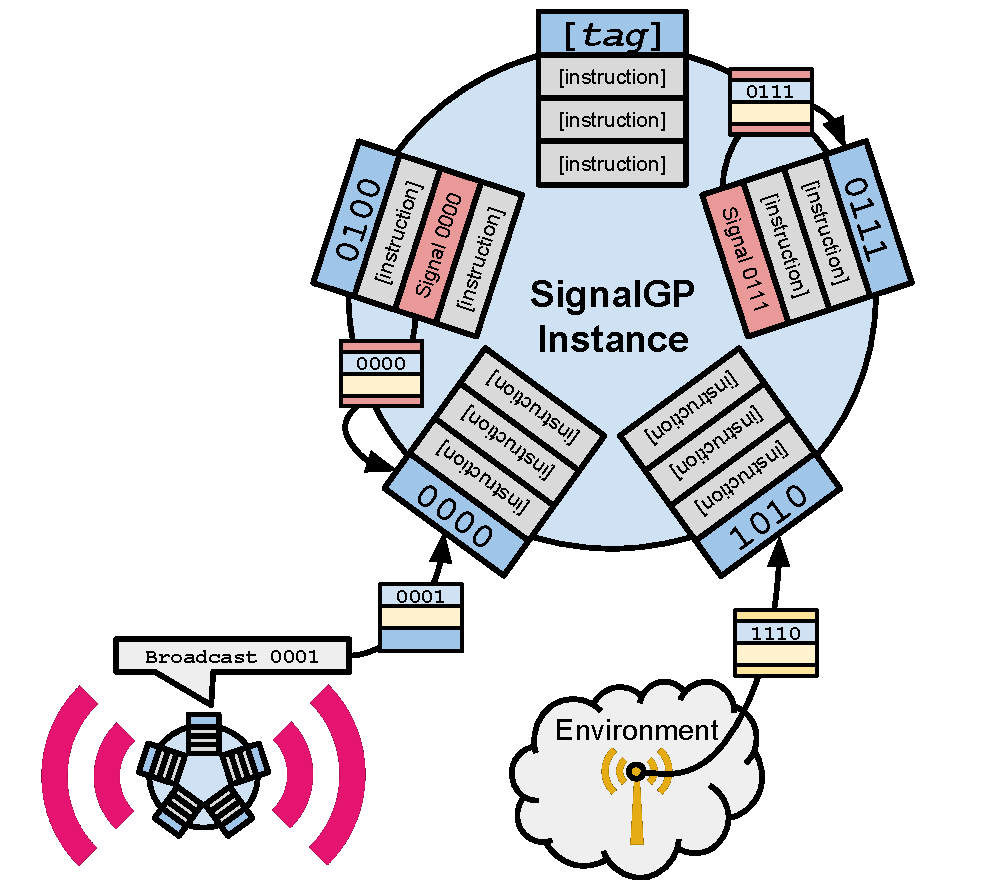
\includegraphics[width=\linewidth]{img/signalgp-cartoon}

\textbf{(A)}Overview of a single SignalGP instance.
SignalGP program modules contain ordered sets of instructions that activate and execute independently in response to tagged signals.
Above, these modules are shown as rectangular lists with bitstring tags protruding from the SignalGP instance.
These signals can originate from any of three sources:
  (1) internally from execution of ``Signal'' instructions within a program's modules,
  (2) from the outside environment, or
  (3) from other agents executing ``Message'' instructions.
Graphic provided courtesy Alexander Lalejini.
\end{minipage}
\begin{minipage}{0.49\textwidth}
  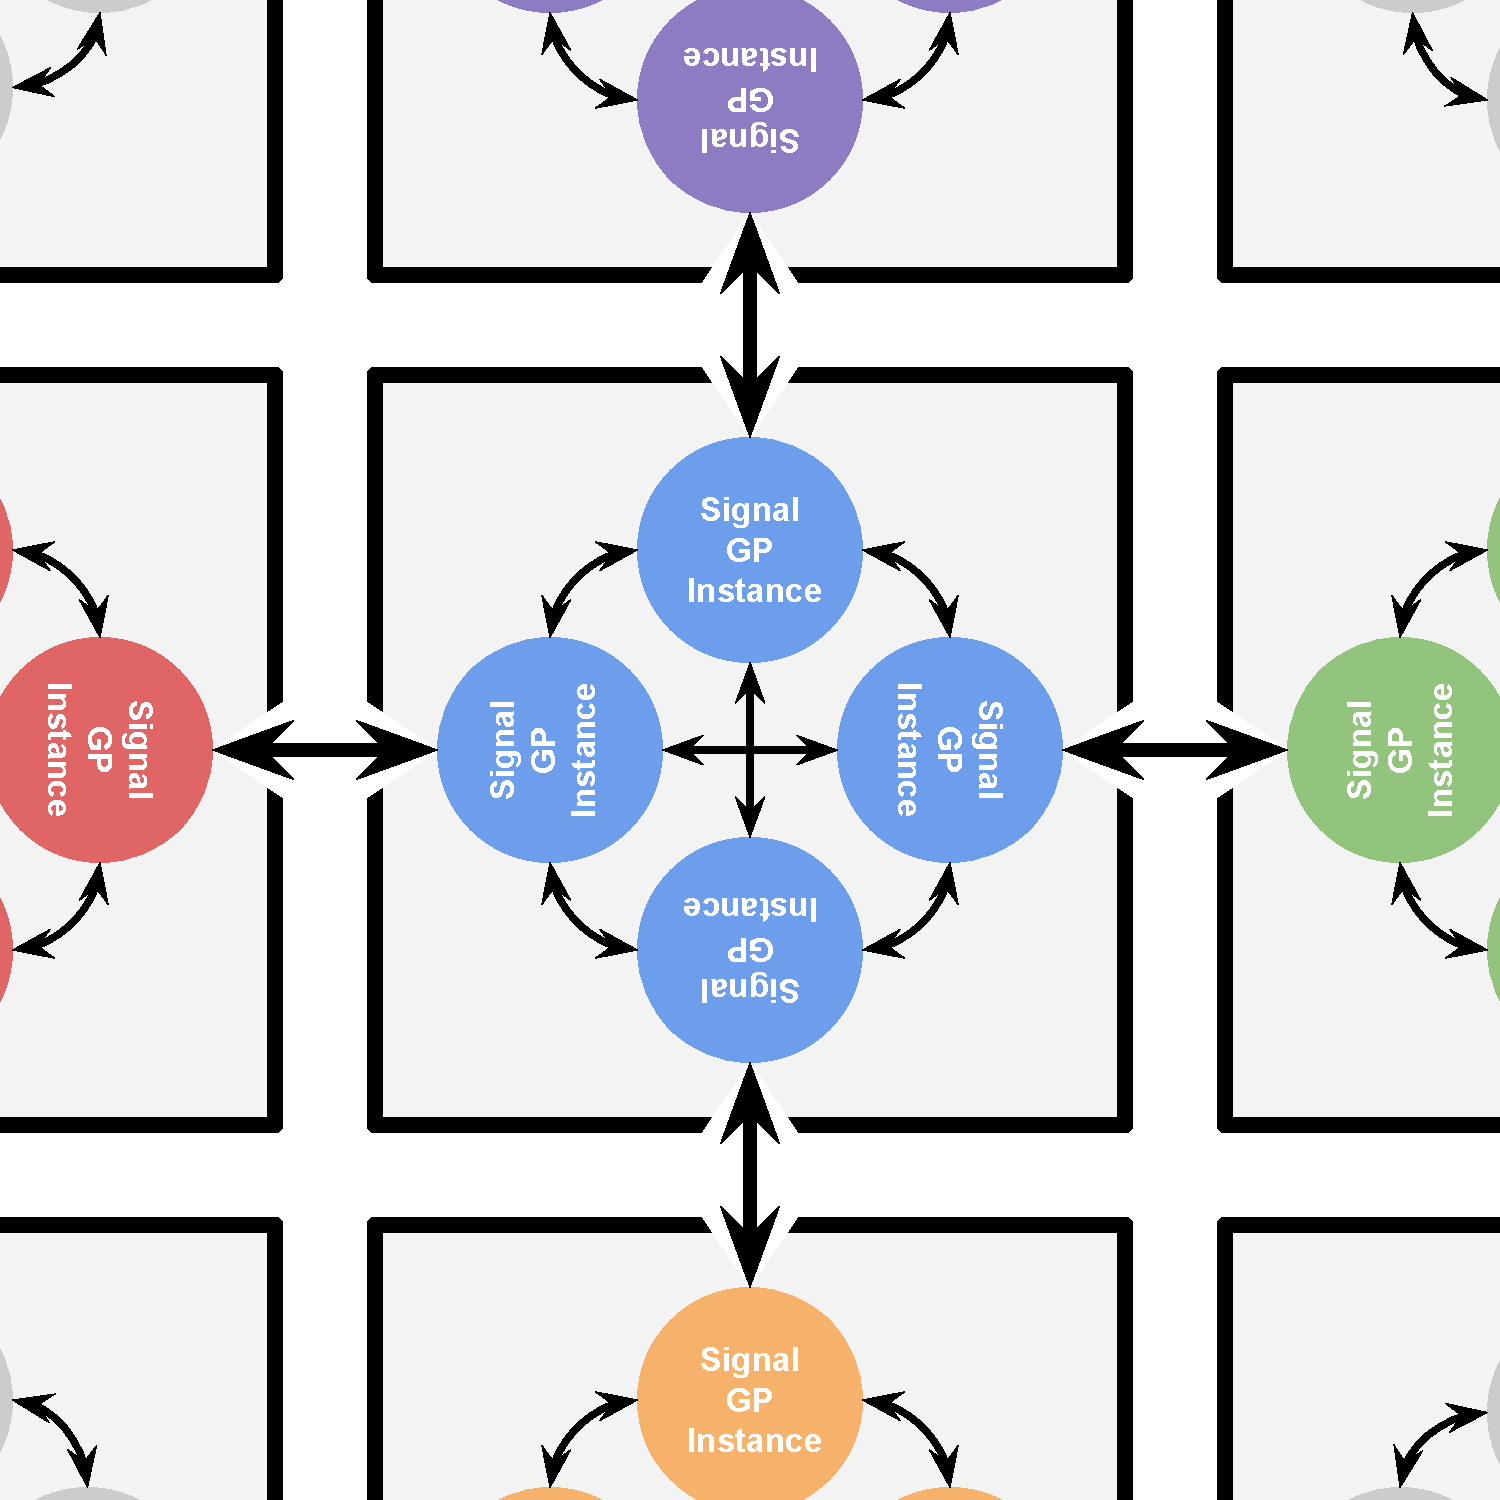
\includegraphics[width=\linewidth]{img/dishtinygp-cartoon}
  \textbf{(B)}
  How individual SignalGP instances are organized into DISHTINY cells.
  Above, DISHTINY cells are depicted as gray squares.
  Each DISHTINY cell is controlled by independent execution of the cell's genetic program on four distinct SignalGP instances, depicted as colored circles.
  Each of four independent instances manages cell behavior with respect to a single cardinal direction: sensing environmental state, receiving intercellular messages, and determining cell actions.
  Above, the special role of each instance is depicted as a reciporical arrow to the neighboring instance in the neighboring cell.
  (All four instances sense non-directional environmental cues and non-directional actions may be taken by any instance.)
  These four instances can communicate with one another via intracellular messaging, indicated above by smaller reciprocal arrows among instances within a cell.
\end{minipage}

\caption{
Schematic illustrations of how an individual SignalGP instance functions and how SignalGP instances control DISHTINY cells.
Execution of cells' genetic programs on SignalGP instances controls cell behavior in our model.
}
\label{fig:signalgp-dishtinygp}
\end{center}
\end{figure*}
